% Options for packages loaded elsewhere
\PassOptionsToPackage{unicode}{hyperref}
\PassOptionsToPackage{hyphens}{url}
\documentclass[
  10pt,
  a4paper,
]{article}
\usepackage{xcolor}
\usepackage[margin=22mm]{geometry}
\usepackage{amsmath,amssymb}
\setcounter{secnumdepth}{-\maxdimen} % remove section numbering
\usepackage{iftex}
\ifPDFTeX
  \usepackage[T1]{fontenc}
  \usepackage[utf8]{inputenc}
  \usepackage{textcomp} % provide euro and other symbols
\else % if luatex or xetex
  \usepackage{unicode-math} % this also loads fontspec
  \defaultfontfeatures{Scale=MatchLowercase}
  \defaultfontfeatures[\rmfamily]{Ligatures=TeX,Scale=1}
\fi
\usepackage{lmodern}
\ifPDFTeX\else
  % xetex/luatex font selection
\fi
% Use upquote if available, for straight quotes in verbatim environments
\IfFileExists{upquote.sty}{\usepackage{upquote}}{}
\IfFileExists{microtype.sty}{% use microtype if available
  \usepackage[]{microtype}
  \UseMicrotypeSet[protrusion]{basicmath} % disable protrusion for tt fonts
}{}
\makeatletter
\@ifundefined{KOMAClassName}{% if non-KOMA class
  \IfFileExists{parskip.sty}{%
    \usepackage{parskip}
  }{% else
    \setlength{\parindent}{0pt}
    \setlength{\parskip}{6pt plus 2pt minus 1pt}}
}{% if KOMA class
  \KOMAoptions{parskip=half}}
\makeatother
\usepackage{graphicx}
\makeatletter
\newsavebox\pandoc@box
\newcommand*\pandocbounded[1]{% scales image to fit in text height/width
  \sbox\pandoc@box{#1}%
  \Gscale@div\@tempa{\textheight}{\dimexpr\ht\pandoc@box+\dp\pandoc@box\relax}%
  \Gscale@div\@tempb{\linewidth}{\wd\pandoc@box}%
  \ifdim\@tempb\p@<\@tempa\p@\let\@tempa\@tempb\fi% select the smaller of both
  \ifdim\@tempa\p@<\p@\scalebox{\@tempa}{\usebox\pandoc@box}%
  \else\usebox{\pandoc@box}%
  \fi%
}
% Set default figure placement to htbp
\def\fps@figure{htbp}
\makeatother
\setlength{\emergencystretch}{3em} % prevent overfull lines
\providecommand{\tightlist}{%
  \setlength{\itemsep}{0pt}\setlength{\parskip}{0pt}}
\usepackage{mathrsfs}
\newcommand{\Log}{\operatorname{Log}}
\usepackage{mathtools}
\usepackage{xurl}
\emergencystretch=3em
\setcounter{tocdepth}{1}
\newcommand{\Beta}{\mathrm{B}}
\DeclareUnicodeCharacter{00B2}{\ensuremath{^2}}
\DeclareUnicodeCharacter{00B1}{\ensuremath{\pm}}
\DeclareUnicodeCharacter{00D7}{\ensuremath{\times}}
\DeclareUnicodeCharacter{2192}{\ensuremath{\to}}
\DeclareUnicodeCharacter{21D2}{\ensuremath{\Rightarrow}}
\DeclareUnicodeCharacter{21A6}{\ensuremath{\mapsto}}
\DeclareUnicodeCharacter{2208}{\ensuremath{\in}}
\DeclareUnicodeCharacter{2209}{\ensuremath{\notin}}
\DeclareUnicodeCharacter{2212}{\ensuremath{-}}
\DeclareUnicodeCharacter{2227}{\ensuremath{\wedge}}
\DeclareUnicodeCharacter{2228}{\ensuremath{\vee}}
\DeclareUnicodeCharacter{2260}{\ensuremath{\ne}}
\DeclareUnicodeCharacter{2264}{\ensuremath{\le}}
\DeclareUnicodeCharacter{2265}{\ensuremath{\ge}}
\DeclareUnicodeCharacter{2297}{\ensuremath{\otimes}}
\DeclareUnicodeCharacter{00B3}{\ensuremath{^3}}
\DeclareUnicodeCharacter{2074}{\ensuremath{^4}}
\DeclareUnicodeCharacter{2076}{\ensuremath{^6}}
\DeclareUnicodeCharacter{03BB}{\ensuremath{\lambda}}
\DeclareUnicodeCharacter{03BC}{\ensuremath{\mu}}
\DeclareUnicodeCharacter{03B5}{\ensuremath{\epsilon}}
\DeclareUnicodeCharacter{03C4}{\ensuremath{\tau}}
\DeclareUnicodeCharacter{03A6}{\ensuremath{\Phi}}
\DeclareUnicodeCharacter{03B1}{\ensuremath{\alpha}}
\DeclareUnicodeCharacter{03C3}{\ensuremath{\sigma}}
\DeclareUnicodeCharacter{03B4}{\ensuremath{\delta}}
\DeclareUnicodeCharacter{03C0}{\ensuremath{\pi}}
\DeclareUnicodeCharacter{039B}{\ensuremath{\Lambda}}
\DeclareUnicodeCharacter{2202}{\ensuremath{\partial}}
\DeclareUnicodeCharacter{0393}{\ensuremath{\Gamma}}
\DeclareUnicodeCharacter{2205}{\ensuremath{\varnothing}}
\DeclareUnicodeCharacter{221E}{\ensuremath{\infty}}
\DeclareUnicodeCharacter{2200}{\ensuremath{\forall}}
\DeclareUnicodeCharacter{00B9}{\ensuremath{^1}}
\DeclareUnicodeCharacter{00B0}{\ensuremath{{}^\circ}}
\DeclareUnicodeCharacter{211D}{\ensuremath{\mathbb{R}}}
\usepackage{bookmark}
\IfFileExists{xurl.sty}{\usepackage{xurl}}{} % add URL line breaks if available
\urlstyle{same}
\hypersetup{
  hidelinks,
  pdfcreator={LaTeX via pandoc}}

\author{}
\date{}

\begin{document}

{
\setcounter{tocdepth}{3}
\tableofcontents
}
\section{The actual heat pairing, its supported endpoints, and mixed
prime
products}\label{the-actual-heat-pairing-its-supported-endpoints-and-mixed-prime-products}

\textbf{Original-zeta receiving calculation.} The working meromorphic
function is the original Riemann zeta, with its full Gamma/endpoints
multiplier and its full trivial-zero and pole divisor retained.
\href{FAITHFUL_THETA_COMPLETION_RETURN.md}{TF1--42} proves the original
labelled theta inverse and the actual heat-image defect.
\href{FAITHFUL_UNCOMPLETED_ZETA_HEAT.md}{UZ1--53} proves every
exceptional-point fibre, jet, original-zeta heat term and reflection
orientation.
\href{ORIGINAL_ZETA_COMPACT_WEIL_RECONSTRUCTION.md}{OZC1--48} rederives
the compact contour and interval operator directly from zeta, including
the left-cutoff Gamma boundary, and specifies exactly which compensated
pairing the bounds concern.
\href{ORIGINAL_ZETA_HEAT_CONTACT_RECONSTRUCTION.md}{OZH1--49} rederives
the actual meromorphic heat, rational signed trace, compact-test domain,
contact drift and full causal arithmetic variation. The raw full divisor
and the compensated Weil receiver are linked by their displayed
correction, not identified. In particular the fixed-test trivial-zero
sum converges exactly at translations at least 1/32 and equals the
earlier R term; at zero translation it requires the proved cutoff
compensation. \href{ORIGINAL_ZETA_CAUCHY_RECONSTRUCTION.md}{OZK1--38}
reconstructs the original signed Cauchy trace, its full Gamma
correction, resonant finite parts, every finite matrix and its index,
and the complete local heat jets. Its invertible map retains the raw
trace and correction separately. These complete receiving proofs govern
the interpretation of the retained auxiliary calculations below.

This calculation uses the original heat family and the full
supported-zero explicit formula. It gives an actual global family of
pairings and computes its arithmetic derivative. Positivity of that
family at time zero is not assumed. All lower support coordinates remain
in the formula.

\subsection{1. Original family and
coordinates}\label{original-family-and-coordinates}

Write \(\xi_R(s)=\tfrac12s(s-1)\pi^{-s/2}\Gamma(s/2)\zeta(s)\). The
original Rodgers--Tao conventions are \[
\begin{aligned}
\Phi(u)&=\sum_{n\ge1}(2\pi^2n^4e^{9u}-3\pi n^2e^{5u})e^{-\pi n^2e^{4u}},\\
H_t(Z)&=\int_0^\infty e^{tu^2}\Phi(u)\cos(Zu)\,du,\\
H_0(Z)&=\tfrac18\xi_R(\tfrac12+iZ/2),\qquad
\partial_tH_t=-\partial_Z^2H_t.
\end{aligned}\tag{HA1}
\] These are the original source equations \texttt{phidef},
\texttt{htdef}, \texttt{hoz}, and the sentence following \texttt{htdef}
in \href{https://arxiv.org/src/1801.05914v5}{Rodgers--Tao,
arXiv:1801.05914v5, author TeX}. Define, retaining the factor 16 and the
coordinate factor \(-2i\), \[
g_t(s)=16H_t(-2i(s-\tfrac12)),\qquad g_0(s)=2\xi_R(s),
\qquad L_t(s)=\frac{\partial_sg_t(s)}{g_t(s)}.
\tag{HA2}
\] The superexponential decrease in (HA1) makes the integral and all its
derivatives converge uniformly on compact subsets of
\(\mathbb C_t\times\mathbb C_s\). For example, on \(|t|\le T,|s|\le R\),
its integrand is bounded by a constant times
\(\exp(Tu^2+2(R+1)u+9u-ce^{4u})\), an integrable function; derivatives
add only polynomial factors in \(u\). It follows by differentiation that
\[
\partial_tg_t=\tfrac14\partial_s^2g_t,\qquad
\partial_tL_t=\tfrac14\partial_s\left(\frac{g_t''}{g_t}\right)
=\tfrac14(L_t''+2L_tL_t').
\tag{HA3}
\] The factor \(1/4\) follows because \((-2i)^2=-4\). For every complex
\(t\), \(g_t(1-s)=g_t(s)\). For real \(t\),
\(g_t(\bar s)=\overline{g_t(s)}\). Thus \[
L_t(1-s)=-L_t(s),\qquad
L_t(\bar s)=\overline{L_t(s)}\quad(t\in\mathbb R).
\tag{HA4}
\] These identities hold wherever the displayed quotients are defined.

\subsection{2. The Cauchy tests in the original Mellin
convention}\label{the-cauchy-tests-in-the-original-mellin-convention}

Let \(z,w\in\mathcal U=\{s:\Re s>1\}\), and put \[
q=w+\bar z-1,\qquad F_z(s)=\frac1{s-z},\qquad
A_{z,w}(s)=F_z^\#(s)F_w(s)
=-\frac1{(s-(1-\bar z))(s-w)},
\tag{HA5}
\] where \(F^\#(s)=\overline{F(1-\bar s)}\). In particular, \(\Re q>1\),
and both poles lie strictly outside the closed critical strip. The exact
original inverse Mellin tests are \[
f_z(u)=-1_{(-\infty,0]}(u)e^{(z-1/2)u},\qquad
h_{z,w}=f_z^\#*f_w,
\tag{HA6}
\] with time-domain involution \(f^\#(u)=\overline{f(-u)}\). Direct
integration gives \[
h_{z,w}(u)=\frac1q
\begin{cases}
e^{-(\bar z-1/2)u},&u\ge0,\\
e^{(w-1/2)u},&u\le0,
\end{cases}
\quad
A_{z,w}(s)=\int_{\mathbb R}h_{z,w}(u)e^{-(s-1/2)u}\,du.
\tag{HA7}
\] The second identity initially holds for \(1-\Re z<\Re s<\Re w\),
including the closed critical strip; it then gives the meromorphic
expression (HA5). The function \(h\) is continuous at zero, and its
derivative jump is exactly \(-1\). Its distributional second derivative
is the sum of two exponentially decreasing functions and \(-\delta_0\).
Neither this atom in the test derivative nor the supported-zero point is
identified with the unsupported element \(\tau\).

The complete extension of the compact-test explicit formula to these
tests is proved in \href{ACTUAL_HEAT_ZERO_DISTRIBUTION_VARIATION.md}{the
global heat zero-distribution calculation}. Here is also the needed
convergence argument. Choose \(d\) strictly between \(1/2\) and
\(\min(\Re z,\Re w)-1/2\). Cut \(h\) off with a smooth function equal to
one on \([-R,R]\) and zero outside \([-R-1,R+1]\), and convolve with a
smooth approximate identity of radius \(\varepsilon_R\le1\), where
\(\varepsilon_R\to0\) as \(R\to\infty\). The resulting smooth compact
tests have uniformly bounded weighted \(L^1\) norms of their value and
first derivative and uniformly bounded weighted total variation of the
second derivative, with weight \(e^{d|u|}\). This follows directly from
(HA7), its derivative jump, the bounded cutoff derivatives and the
compact support of the mollifier. Their transforms therefore obey a
uniform bound \(C/(1+|y|^2)\) for \(0\le\Re s\le1\), by distributional
integration by parts twice. Their pointwise limits give \(A\). The
unconditional zero count \(N(R)=O(R\log(2+R))\), already proved in
SZW25, makes the zero sums uniformly summable. The prime sum is
dominated by \(C\sum\Lambda(n)n^{-1/2-d}\), and the archimedean integral
by \(C\log(2+|y|)/(1+y^2)\). Endpoints converge by the same weighted
\(L^1\) estimate. Thus dominated convergence applies to every term of
SZW25, retaining both endpoints and every support label.

\subsection{3. Exact global pairing and all arithmetic terms at
zero}\label{exact-global-pairing-and-all-arithmetic-terms-at-zero}

Zeros are counted with their multiplicities. The rational zero trace is
\[
K_t(z,w)=\sum_{g_t(\rho)=0}m_\rho A_{z,w}(\rho).
\tag{HA8}
\] For each fixed finite set of \(z,w\) there is a complex time disc
around zero in which no pole of its tests is a zero of \(g_t\). The full
global Hadamard argument in
\href{ACTUAL_HEAT_ZERO_DISTRIBUTION_VARIATION.md}{the zero-distribution
calculation} proves convergence and holomorphic dependence on that disc,
and gives \[
K_t(z,w)=\frac{L_t(w)-L_t(1-\bar z)}q
=\frac{L_t(w)+L_t(\bar z)}q.
\tag{HA9}
\] For real time the numerator is \(L_t(w)+\overline{L_t(z)}\). The
proof can be seen directly from the genus-one logarithmic derivative:
subtract its values at the two poles. The constant term and each
\(1/\rho\) correction cancel; the remaining summand divided by \(q\) is
exactly (HA5) at \(\rho\). Absolute convergence follows from
\(A(\rho)=O(|\rho|^{-2})\) and the uniform zero count. Multiplicities
are retained in this argument.

Introduce three distinct functions on \(\Re s>1\): \[
\begin{aligned}
e_0(s)&=\frac1s+\frac1{s-1},\\
b(s)&=-\tfrac12\log\pi+\tfrac12\psi(s/2),\\
r(s)&=\frac{\zeta'(s)}{\zeta(s)}=-\sum_{n\ge2}\Lambda(n)n^{-s}.
\end{aligned}\qquad L_0=e_0+b+r.
\tag{HA10}
\] The notation \(e_0(s)\) is a scalar logarithmic-derivative function,
not the programme element \(e\). The endpoint, archimedean and
finite-prime values for (HA7) are, separately, \[
\begin{aligned}
E(z,w)&=A_{z,w}(0)+A_{z,w}(1)
=\frac1{w(\bar z-1)}+\frac1{\bar z(w-1)}
=\frac{e_0(w)+\overline{e_0(z)}}q,\\
G(z,w)&=\frac{b(w)+\overline{b(z)}}q,\\
P(z,w)&=\frac1q\sum_{n\ge2}\Lambda(n)(n^{-w}+n^{-\bar z})
=-\frac{r(w)+\overline{r(z)}}q,\\
K_0(z,w)&=E(z,w)+G(z,w)-P(z,w).
\end{aligned}\tag{HA11}
\] The endpoint equality follows by common denominators, and the prime
equality follows from (HA7) in SZW24. For completeness, the Gamma
equality has a direct integral proof. The convergent digamma
representation for \(\Re a>0\) is \[
\psi(a)=-\gamma+\int_0^\infty
\frac{e^{-x}-e^{-ax}}{1-e^{-x}}\,dx.
\tag{HA12}
\] It follows from the logarithmic derivative of Euler's product for
Gamma: expand \((1-e^{-x})^{-1}\), integrate finite partial sums, and
use the cancellation at zero to obtain
\(-\gamma+\sum_{j\ge0}(1/(j+1)-1/(j+a))\). With the original Fourier
convention, the archimedean integral is consequently \[
\begin{aligned}
A_\infty(h)=&-(\gamma+\log\pi)h(0)\\
&+\int_0^\infty\frac{e^{-x}h(0)-\frac12e^{-x/4}(h(x/2)+h(-x/2))}{1-e^{-x}}\,dx.
\end{aligned}\tag{HA13}
\] One may first truncate the \(x\) integral. Fourier inversion then
proves the identity. Passing to the limit is legitimate: at zero the
numerator is \(O(x)\) by the Lipschitz property of \(h\), and at
infinity it decreases exponentially. On the Fourier side, the truncated
integrals are bounded by \(C\log(2+|y|)\), uniformly in the cutoffs. To
verify that bound, split at \(x=1/(1+|y|)\) and at 1 and use
\(|1-\cos(yx/2)|\le\min(2,y^2x^2/8)\). The remaining nonoscillatory
difference is integrable independently of \(y\). The bound on
\(A(1/2+iy)\) proved above supplies domination. Substituting (HA7) in
(HA13) gives (HA11) by (HA12), with every factor \(1/2\) retained.

Let \(L\) now denote the finite support semilattice of SZW, with top
\(1_L\); this is distinct from the function \(L_t(s)\). In the unchanged
vector space with coordinate basis \(\mathbf e_\lambda\), the full
identity is \[
\begin{aligned}
\boldsymbol B_L(z,w)&=E(z,w)\mathbf e_{1_L}
+A_{z,w}(0)\sum_{\lambda\ne1_L}\mathbf e_\lambda,\\
\boldsymbol Z_L(0;z,w)&=K_0(z,w)\mathbf e_{1_L},\\
\boldsymbol D_L(0;z,w)&=(P(z,w)-G(z,w))\mathbf e_{1_L}
+A_{z,w}(0)\sum_{\lambda\ne1_L}\mathbf e_\lambda,\\
\boldsymbol B_L-\boldsymbol Z_L(0)&=\boldsymbol D_L(0).
\end{aligned}\tag{HA14}
\] This is exactly SZW33--34 evaluated on (HA7). In particular, the
lower fixed traces have not been dropped. Summing all coordinates and
projecting to the top coordinate are different maps with the kernels
proved in SZW35--37. The coefficient of each lower coordinate is
generally not a Hermitian form by itself. The Hermitian positivity
question below concerns the full reflected zero trace \(K_0\), as in
SZW32 and SZW38, with (HA14) giving its exact supported arithmetic
realization.

\subsection{4. The actual derivative and its mixed prime
products}\label{the-actual-derivative-and-its-mixed-prime-products}

Set \(a=e_0+b\), and define \(v=a'+a^2\). For \(\Re s>1\), the exact
series is \[
\frac{g_0''}{g_0}(s)
=v(s)+\sum_{n\ge2}\bigl[\Lambda(n)\log n+(\Lambda*\Lambda)(n)-2a(s)\Lambda(n)\bigr]n^{-s},
\tag{HA15}
\] where \((\Lambda*\Lambda)(n)=\sum_{d\mid n}\Lambda(d)\Lambda(n/d)\)
is ordered Dirichlet convolution. Indeed \(g_0''/g_0=L_0'+L_0^2\), and
inserting (HA10) gives (HA15). Each series, each required derivative and
each product converges absolutely and locally uniformly on \(\Re s>1\),
because \(\Lambda(n)\le\log n\) and \(\sum (\log n)^j n^{-c}<\infty\)
for every fixed \(c>1\).

It follows that the genuine time derivative is \[
\begin{aligned}
J(s):=\left.\partial_tL_t(s)\right|_{t=0}
=\frac14v'(s)+\frac14\sum_{n\ge2}C_n(s)n^{-s},\\
C_n(s)=-\Lambda(n)(\log n)^2-(\Lambda*\Lambda)(n)\log n
-2a'(s)\Lambda(n)+2a(s)\Lambda(n)\log n.
\end{aligned}\tag{HA16}
\] This includes the endpoint--Gamma and endpoint--prime cross terms in
\(a\), not merely a heat deformation of the old prime weights. Equations
(HA3) and (HA9) yield the exact global derivative \[
\boxed{\left.\partial_tK_t(z,w)\right|_{t=0}
=\frac{J(w)+\overline{J(z)}}{w+\bar z-1}.}
\tag{HA17}
\] It is a derivative of the actual infinite zero trace, not only a
derivative of a finite set of zeros. The holomorphic finite-pole formula
(HA9) supplies the justification; no unproved interchange with a moving
infinite zero sum is used.

There is a useful exact distinction among arithmetic indices. If
\(n=p^k\), then \[
\Lambda(n)\log n+(\Lambda*\Lambda)(n)
=(2k-1)(\log p)^2.
\tag{HA18}
\] The \(k-1\) ordered proper prime-power factorizations give the
convolution. If \(n=p^\alpha q^\beta\), where \(p\ne q\) and
\(\alpha,\beta\ge1\), then \[
\Lambda(n)=0,\quad (\Lambda*\Lambda)(n)=2\log p\log q,
\quad \frac14C_n(s)=-\frac12\log p\log q\log(p^\alpha q^\beta).
\tag{HA19}
\] These are the two possible ordered factorizations into prime powers.
With three or more distinct prime divisors both functions vanish. Thus
the first actual heat derivative already contains products of two
distinct prime contributions. Formula (HA19) does not arise from
replacing an ordinary prime by a new numerical norm for supported zero.
It is forced by the nonlinear term \(2L_0L_0'\) in the exact evolution.

To retain the whole support vector through this calculation, let
\(\Lambda_t(s)=g_t(s)/(s(s-1))\). At real time close to zero this
function has simple poles at zero and one, since \(g_0(0)=g_0(1)=1\) and
compact continuity keeps both values nonzero. Its logarithmic derivative
is \(L_t-e_0\), with residue \(-1\) at each pole. Their residues as
poles of \(\Lambda_t\) itself are \(-g_t(0)\) and \(g_t(1)\), and may
vary; these two statements are distinct.

The logarithmic-divisor receiver at time \(t\) therefore has unchanged
fixed endpoint weights and explicitly computed top coefficient \[
\begin{aligned}
\boldsymbol Z_L(t)&=K_t\mathbf e_{1_L},\\
\boldsymbol D_L(t)&=\left(E-\frac{L_t(w)+L_t(\bar z)}q\right)\mathbf e_{1_L}
+A_{z,w}(0)\sum_{\lambda\ne1_L}\mathbf e_\lambda,\\
\boldsymbol B_L-\boldsymbol Z_L(t)&=\boldsymbol D_L(t),\\
\dot{\boldsymbol D}_L(0)&=-\frac{J(w)+\overline{J(z)}}q\mathbf e_{1_L},
\qquad \dot{\boldsymbol B}_L=0.
\end{aligned}\tag{HA20}
\] Here the first two lines are evaluated from the actual meromorphic
heat function and its divisor. At zero, (HA11) identifies them with the
original arithmetic formula; (HA16) computes their arithmetic first
variation. No Euler product for \(g_t\) at nonzero time, or new
theta-cohomology identification at such time, is asserted. The lower
fixed distributions are the same explicit representations used in SZW,
and their zero derivative is a calculation for these fixed tests, not a
deletion of those distributions.

\subsection{5. Exact relation to a colliding
infinitesimal}\label{exact-relation-to-a-colliding-infinitesimal}

Fix any actual zero \(\rho\) of \(g_0\), of multiplicity \(m\), and
write \(g_0(s)=(s-\rho)^m u(s)\), \(u(\rho)\ne0\). On a small circle
enclosing just this cluster, the residue theorem gives its weighted
trace. Differentiating that fixed contour using (HA3) gives \[
\left.\partial_t Z_{\rho,t}(A)\right|_0
=-\frac{m(m-1)}4 A''(\rho)
-\frac m2\frac{u'(\rho)}{u(\rho)}A'(\rho).
\tag{HA21}
\] For proof, \(g_0''/(4g_0)\) has principal part
\(\frac{m(m-1)}4(s-\rho)^{-2}+\frac m2(u'/u)(\rho)(s-\rho)^{-1}\). Its
derivative has residue against \(A\) equal to the displayed expression.
The contour derivative exists without choosing or differentiating
individual colliding roots. Formula (HA21) retains the full analytic
unit.

For a critical-line zero \(\rho=1-\bar\rho\), take local tests \(F,G\)
vanishing at \(\rho\) and put \(A=F^\#G\). Then \(A'(\rho)=0\) and
\(A''(\rho)=-2\overline{F'(\rho)}G'(\rho)\). Hence \[
\left.\partial_t Z_{\rho,t}(F^\#G)\right|_0
=\frac{m(m-1)}2\overline{F'(\rho)}G'(\rho).
\tag{HA22}
\] This is the exact positive first response on the first vanishing-jet
layer of a critical collision. At an exchanged pair \(\rho,\rho^\#\),
the same calculation gives the cross pairing of the two derivative
values; its Gram matrix is a positive multiple of
\(\begin{psmallmatrix}0&1\\1&0\end{psmallmatrix}\), provided both tests
vanish at both points and \(m\ge2\). Thus the actual first response
preserves the distinction between a critical fixed point and an
exchanged pair. If \(m=1\), this particular first-jet response vanishes,
while (HA21) still retains the unit-dependent term for arbitrary tests.

For a finite rational test span \(F=\sum_j c_jF_{z_j}\), the global
quadratic form and derivative are exactly \[
Z_t(F^\#F)=\sum_{i,j}\bar c_iK_t(z_i,z_j)c_j,
\qquad
\left.\partial_t Z_t(F^\#F)\right|_0
=\sum_{i,j}\bar c_i\frac{J(z_j)+\overline{J(z_i)}}{z_j+\bar z_i-1}c_j.
\tag{HA23}
\] Every zero and every endpoint is retained by (HA8) and (HA14). A sign
on (HA22), or on a coefficient of (HA19), does not assign a sign to
(HA23). The complete criterion for the latter family at zero is proved
in \href{CAUCHY_WEIL_POSITIVITY_CRITERION.md}{Cauchy--Weil positivity}.

\subsection{6. A positive actual diagonal response and its precise
scope}\label{a-positive-actual-diagonal-response-and-its-precise-scope}

The kernel permits an unconditional sign calculation on the real
diagonal. For every real \(t\), \(\sigma>1\), put \(v=\sigma-1/2>0\) and
give \([0,\infty)\) the probability measure \[
d\mu_{t,v}(u)=\frac{e^{tu^2}\Phi(u)\cosh(2vu)\,du}{\int_0^\infty e^{ty^2}\Phi(y)\cosh(2vy)\,dy}.
\tag{HA24}
\] The measure is positive: every summand of \(\Phi(u)\) is
\(\pi n^2e^{5u}(2\pi n^2e^{4u}-3)e^{-\pi n^2e^{4u}}>0\) for \(u\ge0\).
Its density is strictly positive and all moments exist. Differentiation
of the actual integral (HA1), with the compact domination already
proved, gives \[
L_t(\sigma)=2\,\mathbb E_{\mu_{t,v}}[u\tanh(2vu)]>0,
\quad
\partial_tL_t(\sigma)=2\operatorname{Cov}_{\mu_{t,v}}(u^2,u\tanh(2vu))>0.
\tag{HA25}
\] For the second identity differentiate a normalized integral. Its
strict sign follows from \[
2\operatorname{Cov}(f,g)=\iint(f(u)-f(y))(g(u)-g(y))\,d\mu(u)d\mu(y).
\tag{HA26}
\] Both \(u^2\) and \(u\tanh(2vu)\) are strictly increasing on
\((0,\infty)\). The integrand is positive away from the diagonal, and
the positive continuous density gives positive mass to two disjoint
intervals. Thus the covariance is strictly positive, not merely
nonnegative.

Consequently \(K_t(\sigma,\sigma)=2L_t(\sigma)/(2\sigma-1)>0\) and its
actual time derivative is strictly positive for every real time. The
rational trace identity applies at every such fixed real time: its two
real poles are not zeros because the same positive integral makes
\(g_t(\sigma)>0\) and reflection gives \(g_t(1-\sigma)>0\). Its growth
and Hadamard argument are local on arbitrary bounded time intervals.
This calculation keeps the original measure and all coefficients; it is
not positivity imposed on an auxiliary model.

The result identifies precisely what the real diagonal observes. It does
not control the off-diagonal matrix entries. In particular, positive
values and a positive first derivative on this diagonal also occur at
negative heat times. Rodgers--Tao's original Theorem \texttt{main},
together with the defining real-zero threshold stated in their
introduction, proves that those negative times do have nonreal zeros in
the original \(Z\) coordinate. Thus this actual diagonal positivity is
strictly weaker than real-rootedness of the actual heat family. The
complete matrix criterion retains the missing off-diagonal data.

\subsection{Sources and exact programme
maps}\label{sources-and-exact-programme-maps}

The human heat source is Brad Rodgers and Terence Tao, \emph{The de
Bruijn--Newman constant is non-negative}, arXiv:1801.05914v5, original
author source \texttt{fmp-\allowbreak{}template.\allowbreak{}tex}, equations \texttt{hoz},
\texttt{sas}, \texttt{phidef}, \texttt{htdef}. The original archive is
retained intact. The programme uses the minus-exponent Mellin convention
of
\href{https://github.com/KokunoYumeto/zeta-function-research-reader/blob/5a89872598df0902b7c1393cf8e4692ca3010a95/workbenches/splitzero-tandem/branches/tau-zero-prime-positivity/SUPPORTED_ZERO_PRIME_WEIL_DERIVATION.md}{SZW19--SZW38},
including its proof of the full explicit formula and every labelled
trace. Its human explicit-formula source is Alain Connes, \emph{Trace
formula in noncommutative geometry and the zeros of the Riemann zeta
function}, Appendix II, Theorem 6, as read and applied there. The
current finite-pole heat trace, the matrix criterion and the arithmetic
calculation have complete separate proofs linked above; none of those
links identifies a pending result as an already published edition.

\subsection{Exact formula diagram}\label{exact-formula-diagram}

\begin{figure}
\centering
\pandocbounded{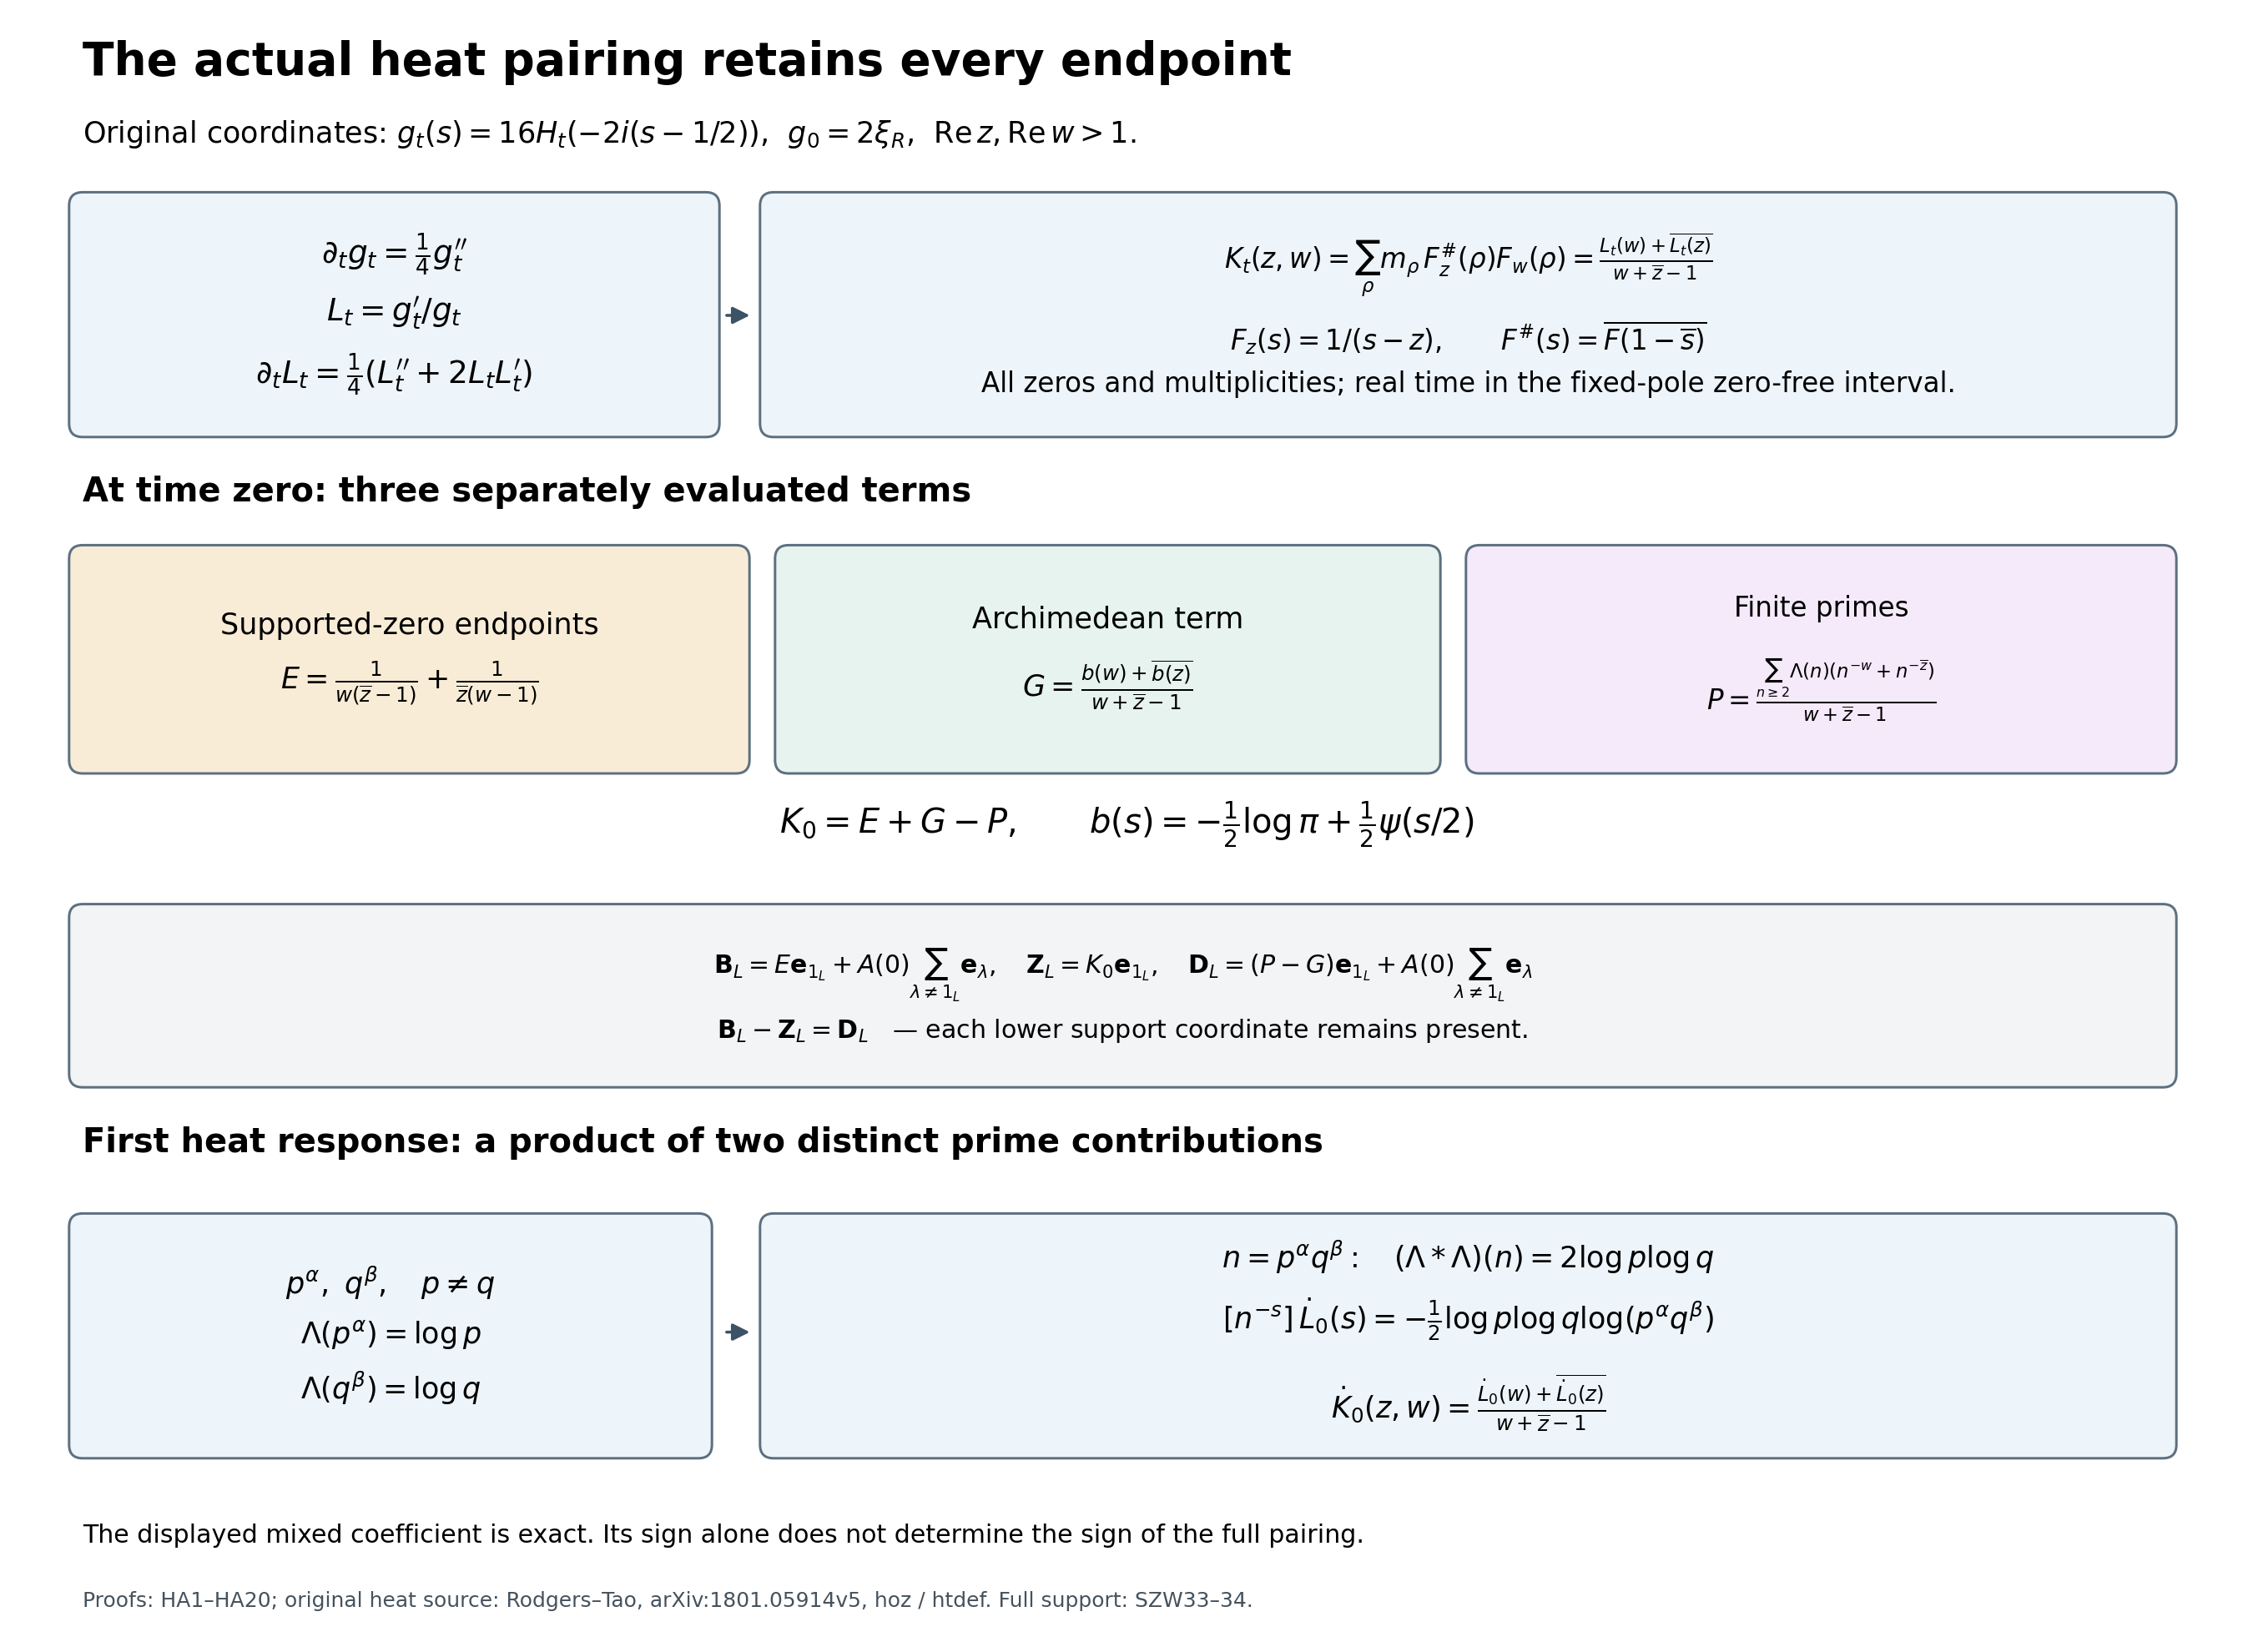
\includegraphics[keepaspectratio,alt={The actual heat coordinates, complete supported arithmetic identity, and first mixed-prime coefficient. Every constant and support coordinate is retained; full proofs HA1--HA20. Here A=F\_z sharp times F\_w as defined in HA5.}]{heat_cauchy_supported_arithmetic.png}}
\caption{The actual heat coordinates, complete supported arithmetic
identity, and first mixed-prime coefficient. Every constant and support
coordinate is retained; full proofs HA1--HA20. Here A=F\_z sharp times
F\_w as defined in HA5.}
\end{figure}

\begin{figure}
\centering
\pandocbounded{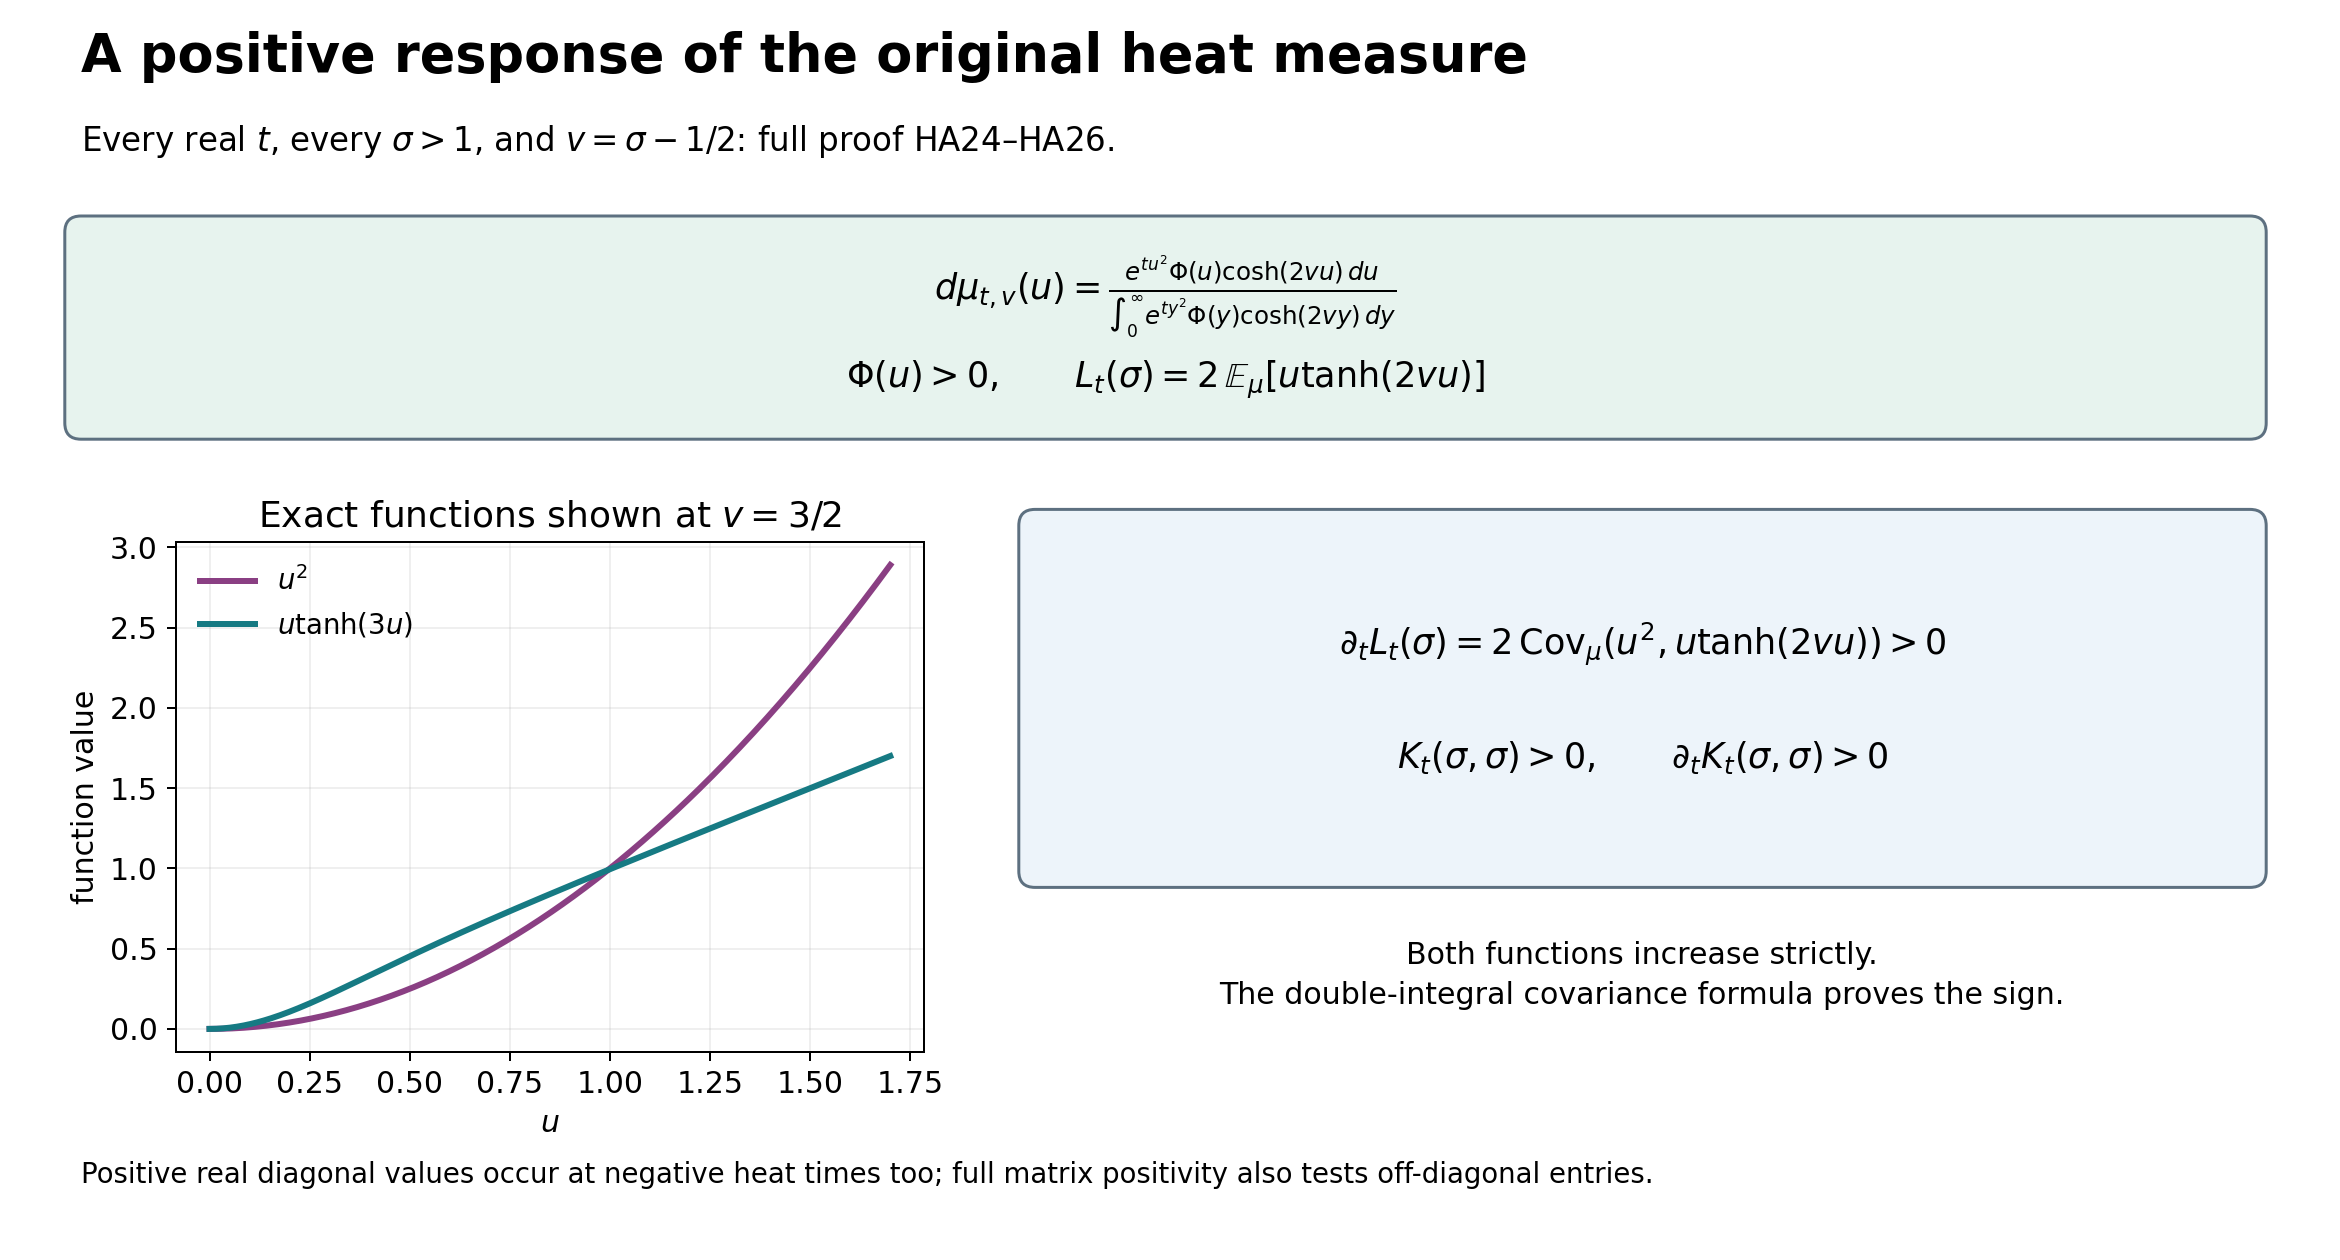
\includegraphics[keepaspectratio,alt={The original positive heat measure and the strict covariance calculation. The two plotted functions are shown at the stated value v=3/2; the theorem and exact integral hold for every v=sigma−1/2 with sigma greater than one. Full proof HA24--HA26.}]{heat_real_diagonal_covariance.png}}
\caption{The original positive heat measure and the strict covariance
calculation. The two plotted functions are shown at the stated value
v=3/2; the theorem and exact integral hold for every v=sigma−1/2 with
sigma greater than one. Full proof HA24--HA26.}
\end{figure}

\subsection{Exact full-form
continuation}\label{exact-full-form-continuation}

The \href{CAUCHY_REFLECTION_INDEX_DERIVATION.md}{reflection-index
theorem, NI1--32}, calculates the signed index of every complete Cauchy
coefficient tail. The
\href{FINITE_JET_COMPLEMENT_AND_HEAT_TRUNCATION.md}{finite-jet and
endpoint proof, FJ1--29}, preserves the exact finite jets while proving
density on the remaining zeros, derives the full exterior index and
tail, and calculates the second and third actual heat coefficients. All
supported endpoints remain explicit. These results identify the
remaining sign problem without asserting its resolution.

\subsection{One fixed primitive test and the entire prime
window}\label{one-fixed-primitive-test-and-the-entire-prime-window}

The \href{PRIME_PROJECTOR_MOBIUS_DERIVATION.md}{prime-operator
calculation}, PM1--41, proves both distinct Fourier support corrections
and their exact map into the full Weil formula. The
\href{PRIMITIVE_SHORT_SUPPORT_DERIVATION.md}{local estimate}, PS1--21,
gives a positive translation-difference remainder. The
\href{UNIVERSAL_PRIMITIVE_TRANSLATION_CRITERION.md}{fixed-test proof},
UP1--35, constructs one compact test whose transform is nonzero at every
possible off-critical zero. The
\href{PRIMITIVE_PRIME_WINDOW_DERIVATION.md}{complete arithmetic
calculation}, PW1--22, expresses its entire translated correlation
through a fixed-width prime window and an explicit archimedean
remainder. Its boundedness is equivalent to RH; that bound remains
unresolved. All boundary coordinates and supported-zero labels remain
explicit.

\subsection{Actual positive-real-time
continuation}\label{actual-positive-real-time-continuation}

The complete \href{REAL_TIME_HEAT_TRACE_DERIVATION.md}{real-time proof},
RT1--30, strengthens the compact-test variation in this edition: the
whole zero trace is smooth for the original real heat time t at least
zero, with actual right derivatives at zero. RT16 identifies its first
derivative with the full causal arithmetic distribution, and RT20--27
constructs every higher meromorphic derivative receiver. The contact
comparison retains the unit and inter-zero terms. These results do not
assert a common zero strip for negative or complex time and do not prove
the remaining RH inequality. All original supported carriers remain
present.

\end{document}
